\documentclass[12pt,a4paper]{article}

% === Packages ===
\usepackage[utf8]{inputenc}
\usepackage[romanian]{babel}
\usepackage[T1]{fontenc}
\usepackage{geometry}
\usepackage{graphicx}
\usepackage{amsmath,amsfonts,amssymb}
\usepackage{listings}
\usepackage{xcolor}
\usepackage{hyperref}
\usepackage{booktabs}
\usepackage{float}
\usepackage{tikz}
\usetikzlibrary{shapes,arrows,positioning}
\usepackage{fancyhdr}
\usepackage{titlesec}
\usepackage{tocloft}
\usepackage{enumitem}
\usepackage{caption}
\usepackage{subcaption}
\usepackage{multirow}
\usepackage{array}
\usepackage{longtable}

% === Page Setup ===
\geometry{
    left=2.5cm,
    right=2.5cm,
    top=2.5cm,
    bottom=2.5cm
}

% === Header/Footer ===
\pagestyle{fancy}
\fancyhf{}
\fancyhead[L]{Proiect Criptografie}
\fancyhead[R]{Simulare One-Time Pad}
\fancyfoot[C]{\thepage}
\renewcommand{\headrulewidth}{0.4pt}
\renewcommand{\footrulewidth}{0.4pt}

% === Colors ===
\definecolor{codegreen}{rgb}{0,0.6,0}
\definecolor{codegray}{rgb}{0.5,0.5,0.5}
\definecolor{codepurple}{rgb}{0.58,0,0.82}
\definecolor{backcolour}{rgb}{0.95,0.95,0.92}
\definecolor{linkblue}{RGB}{0,0,180}

% === Hyperref Setup ===
\hypersetup{
    colorlinks=true,
    linkcolor=linkblue,
    filecolor=magenta,
    urlcolor=cyan,
    pdftitle={Proiect Criptografie - OTP},
    pdfauthor={Student},
}

% === Code Listings ===
\lstdefinestyle{gostyle}{
    backgroundcolor=\color{backcolour},
    commentstyle=\color{codegreen},
    keywordstyle=\color{magenta},
    numberstyle=\tiny\color{codegray},
    stringstyle=\color{codepurple},
    basicstyle=\ttfamily\footnotesize,
    breakatwhitespace=false,
    breaklines=true,
    captionpos=b,
    keepspaces=true,
    numbers=left,
    numbersep=5pt,
    showspaces=false,
    showstringspaces=false,
    showtabs=false,
    tabsize=2,
    frame=single
}
\lstset{style=gostyle}

% === Title Formatting ===
\titleformat{\section}
    {\normalfont\Large\bfseries}{\thesection}{1em}{}
\titleformat{\subsection}
    {\normalfont\large\bfseries}{\thesubsection}{1em}{}

% === Document Start ===
\begin{document}

% === Title Page ===
\begin{titlepage}
    \centering
    \vspace*{2cm}

    {\scshape\LARGE Universitatea \par}
    {\scshape\Large Facultatea de Informatică\par}

    \vspace{2cm}

    {\Huge\bfseries Proiect Criptografie\par}
    \vspace{0.5cm}
    {\LARGE\bfseries Simularea unui Mecanism\\One-Time Pad (OTP)\par}

    \vspace{3cm}

    \begin{minipage}{0.4\textwidth}
        \begin{flushleft}
            \textbf{Student:}\\
            Nume Prenume\\
            Grupa: XXX
        \end{flushleft}
    \end{minipage}
    \begin{minipage}{0.4\textwidth}
        \begin{flushright}
            \textbf{Coordonator:}\\
            Prof. Dr. Nume\\
            Departamentul de Informatică
        \end{flushright}
    \end{minipage}

    \vfill

    {\large Anul Universitar 2024-2025\par}
\end{titlepage}

% === Table of Contents ===
\tableofcontents
\newpage

% ============================================================
\section{Introducere}
% ============================================================

\subsection{Context și Motivație}

Criptografia reprezintă știința și practica comunicării securizate în prezența adversarilor. Într-o lume din ce în ce mai digitalizată, securitatea informației a devenit o necesitate fundamentală pentru protejarea datelor personale, tranzacțiilor financiare și comunicațiilor sensibile.

Acest proiect se concentrează pe implementarea și demonstrarea algoritmului \textbf{One-Time Pad (OTP)} - singurul sistem criptografic demonstrat matematic ca având securitate perfectă de către Claude Shannon în 1949.

\subsection{Obiective}

Obiectivele principale ale acestui proiect sunt:

\begin{enumerate}[label=\arabic*.]
    \item Înțelegerea principiilor fundamentale ale criptografiei simetrice
    \item Implementarea algoritmului One-Time Pad
    \item Demonstrarea operației XOR pentru criptare și decriptare
    \item Generarea cheilor criptografic securizate folosind \texttt{crypto/rand}
    \item Afișarea mesajului în diferite formate (ASCII, hexazecimal)
    \item Verificarea că decriptarea produce mesajul original
    \item Salvarea cheii și mesajului criptat în fișiere (opțional)
\end{enumerate}

\subsection{Structura Proiectului}

Proiectul este organizat astfel:
\begin{itemize}
    \item \textbf{Secțiunea 2}: Fundamente teoretice ale criptografiei
    \item \textbf{Secțiunea 3}: One-Time Pad - teorie și principii
    \item \textbf{Secțiunea 4}: Operația XOR
    \item \textbf{Secțiunea 5}: Implementarea aplicației
    \item \textbf{Secțiunea 6}: Concluzii
\end{itemize}

% ============================================================
\section{Fundamente Teoretice}
% ============================================================

\subsection{Terminologie Criptografică}

\begin{table}[H]
\centering
\caption{Termeni fundamentali în criptografie}
\begin{tabular}{|l|p{10cm}|}
\hline
\textbf{Termen} & \textbf{Definiție} \\
\hline
Plaintext (M) & Mesajul original, în formă citibilă \\
\hline
Ciphertext (C) & Mesajul criptat, rezultatul procesului de criptare \\
\hline
Key (K) & Cheia secretă folosită pentru criptare/decriptare \\
\hline
Encryption & Procesul de transformare: $E_K(M) = C$ \\
\hline
Decryption & Procesul invers: $D_K(C) = M$ \\
\hline
\end{tabular}
\end{table}

\subsection{Criptarea Simetrică}

One-Time Pad este un sistem de criptare simetrică, ceea ce înseamnă că:
\begin{itemize}
    \item Utilizează \textbf{aceeași cheie} pentru criptare și decriptare
    \item Avantaje: rapiditate, eficiență computațională
    \item Dezavantaje: problema distribuției cheilor
\end{itemize}

\subsection{Principiul lui Kerckhoffs}

Auguste Kerckhoffs a formulat în 1883 un principiu fundamental:

\begin{quote}
    \textit{"Un sistem criptografic trebuie să fie securizat chiar dacă totul despre sistem, cu excepția cheii, este de cunoștință publică."}
\end{quote}

Acest principiu este esențial în criptografia modernă - securitatea trebuie să se bazeze exclusiv pe secretul cheii, nu pe obscuritatea algoritmului.

% ============================================================
\section{One-Time Pad (OTP)}
% ============================================================

\subsection{Prezentare Generală}

One-Time Pad, inventat de Gilbert Vernam în 1917, este singurul sistem criptografic cu \textbf{securitate perfectă demonstrată matematic}. Claude Shannon a demonstrat acest lucru în lucrarea sa fundamentală din 1949, "Communication Theory of Secrecy Systems".

\subsection{Principiul de Funcționare}

OTP funcționează prin combinarea fiecărui byte din mesaj cu byte-ul corespunzător din cheie, folosind operația XOR (sau exclusiv).

\subsubsection{Formula Matematică}

\begin{equation}
    C_i = M_i \oplus K_i \quad \text{(Criptare)}
\end{equation}

\begin{equation}
    M_i = C_i \oplus K_i \quad \text{(Decriptare)}
\end{equation}

unde:
\begin{itemize}
    \item $C_i$ = byte-ul $i$ din ciphertext
    \item $M_i$ = byte-ul $i$ din mesaj
    \item $K_i$ = byte-ul $i$ din cheie
    \item $\oplus$ = operația XOR
\end{itemize}

\subsection{Condiții pentru Securitate Perfectă}

Pentru ca OTP să ofere securitate perfectă, trebuie respectate strict următoarele condiții:

\begin{enumerate}
    \item \textbf{Aleatorietate completă}: Cheia trebuie să fie generată folosind un generator de numere aleatoare criptografic securizat (CSPRNG)
    \item \textbf{Lungime egală}: Cheia trebuie să aibă cel puțin lungimea mesajului
    \item \textbf{Utilizare unică}: Cheia nu trebuie folosită niciodată de două ori
    \item \textbf{Secret}: Cheia trebuie păstrată secretă și distribuită în siguranță
\end{enumerate}

\subsection{Demonstrația Securității Perfecte}

Shannon a demonstrat că un sistem are securitate perfectă dacă:

\begin{equation}
    P(M|C) = P(M)
\end{equation}

Adică, probabilitatea unui mesaj $M$ dat ciphertextul $C$ este egală cu probabilitatea a priori a mesajului. Cu alte cuvinte, \textbf{ciphertextul nu oferă nicio informație despre plaintext}.

Pentru OTP, dacă toate condițiile sunt respectate:
\begin{itemize}
    \item Pentru orice ciphertext $C$, orice mesaj $M$ de aceeași lungime este la fel de probabil
    \item Un atacator cu putere de calcul infinită nu poate determina mesajul original
\end{itemize}

\subsection{Pericolul Reutilizării Cheii}

Reutilizarea cheii este cea mai gravă vulnerabilitate a OTP. Dacă aceeași cheie $K$ este folosită pentru două mesaje diferite:

\begin{align}
    C_1 &= M_1 \oplus K \\
    C_2 &= M_2 \oplus K \\
    C_1 \oplus C_2 &= (M_1 \oplus K) \oplus (M_2 \oplus K) = M_1 \oplus M_2
\end{align}

Rezultatul $M_1 \oplus M_2$ permite atacuri bazate pe:
\begin{itemize}
    \item Analiza de frecvență
    \item Crib dragging (ghicirea cuvintelor comune)
    \item Pattern matching
\end{itemize}

\textbf{Exemplu istoric}: Proiectul VENONA al NSA a spart mesaje sovietice tocmai datorită reutilizării cheilor OTP în anii 1940.

% ============================================================
\section{Operația XOR}
% ============================================================

\subsection{Tabelul de Adevăr}

Operația XOR (sau exclusiv) este fundamentală pentru OTP:

\begin{table}[H]
\centering
\caption{Tabelul de adevăr pentru operația XOR}
\begin{tabular}{|c|c|c|}
\hline
\textbf{A} & \textbf{B} & \textbf{A $\oplus$ B} \\
\hline
0 & 0 & 0 \\
0 & 1 & 1 \\
1 & 0 & 1 \\
1 & 1 & 0 \\
\hline
\end{tabular}
\end{table}

\subsection{Proprietăți Importante}

\begin{enumerate}
    \item \textbf{Comutativitate}: $A \oplus B = B \oplus A$
    \item \textbf{Asociativitate}: $(A \oplus B) \oplus C = A \oplus (B \oplus C)$
    \item \textbf{Identitate}: $A \oplus 0 = A$
    \item \textbf{Auto-inversă}: $A \oplus A = 0$
    \item \textbf{Reversibilitate}: $(A \oplus B) \oplus B = A$
\end{enumerate}

Proprietatea de reversibilitate este esențială pentru OTP: aplicând XOR cu aceeași cheie, putem recupera mesajul original.

\subsection{Exemplu Pas cu Pas}

Să luăm caracterul 'A' (cod ASCII 65, binar 01000001) și o cheie aleatorie 10101010:

\begin{verbatim}
Mesaj (A):    01000001
Cheie:        10101010
              --------
Criptat:      11101011

Criptat:      11101011
Cheie:        10101010
              --------
Decriptat:    01000001 = 'A'
\end{verbatim}

% ============================================================
\section{Implementarea Aplicației}
% ============================================================

\subsection{Arhitectura}

Aplicația este construită folosind o arhitectură client-side (browser):

\begin{figure}[H]
\centering
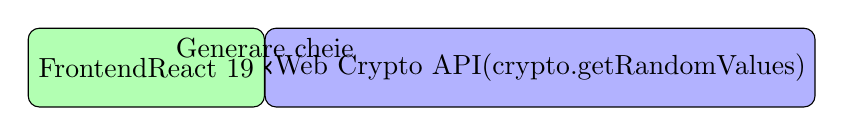
\begin{tikzpicture}[
    node distance=2cm,
    box/.style={draw, rectangle, rounded corners, minimum width=3cm, minimum height=1cm}
]
    \node[box, fill=green!30] (frontend) {Frontend\\React 19};
    \node[box, fill=blue!30, right of=frontend, xshift=3cm] (crypto) {Web Crypto API\\(crypto.getRandomValues)};

    \draw[->, thick] (frontend) -- node[above] {Generare cheie} (crypto);
\end{tikzpicture}
\caption{Arhitectura aplicației}
\end{figure}

\subsection{Tehnologii Utilizate}

\begin{itemize}
    \item \textbf{Frontend}: React 19 + Tailwind CSS
        \begin{itemize}
            \item \texttt{crypto.getRandomValues()} - generare cheie aleatorie
            \item Hooks (useState, useCallback) pentru state management
            \item Tailwind CSS pentru stilizare
        \end{itemize}
\end{itemize}

\subsection{Structura Proiectului}

\begin{verbatim}
OTP-Project/
├── frontend-react/
│   └── src/
│       ├── App.jsx            # Componenta principală
│       └── components/
│           └── OTPSimulator.jsx  # Simulatorul OTP
├── docs/
│   ├── presentation/
│   │   └── presentation.tex
│   └── report/
│       └── project_report.tex
└── README.md
\end{verbatim}

\subsection{Implementare OTP în JavaScript}

\begin{lstlisting}[language=JavaScript, caption=Funcții principale OTP]
// generare cheie aleatorie cu crypto.getRandomValues
const generateKey = (length) => {
  const key = new Uint8Array(length)
  crypto.getRandomValues(key)
  return key
}

// operatia xor intre mesaj si cheie
const xorEncrypt = (messageBytes, keyBytes) => {
  const result = new Uint8Array(messageBytes.length)
  for (let i = 0; i < messageBytes.length; i++) {
    result[i] = messageBytes[i] ^ keyBytes[i]
  }
  return result
}

// conversie bytes la hex pentru afisare
const bytesToHex = (bytes) => {
  return Array.from(bytes)
    .map(b => b.toString(16).padStart(2, '0').toUpperCase())
    .join(' ')
}
\end{lstlisting}

\textbf{Puncte importante în implementare:}
\begin{itemize}
    \item Folosirea \texttt{crypto.getRandomValues()} pentru generarea cheilor (echivalent cu \texttt{crypto/rand} din Go)
    \item Verificarea lungimii cheii față de mesaj
    \item Afișarea în multiple formate (text, ASCII, hex)
\end{itemize}

\subsection{Funcționalități Implementate}

Aplicația oferă următoarele funcționalități:

\begin{enumerate}
    \item \textbf{Input mesaj}: Utilizatorul introduce un mesaj text
    \item \textbf{Generare cheie}: Se generează o cheie aleatorie de lungimea mesajului
    \item \textbf{Criptare XOR}: Mesajul este criptat folosind operația XOR
    \item \textbf{Afișare rezultate}:
        \begin{itemize}
            \item Mesaj original: text, coduri ASCII, hexazecimal
            \item Cheie OTP: hexazecimal
            \item Mesaj criptat: hexazecimal
            \item Mesaj decriptat: text, coduri ASCII, hexazecimal
        \end{itemize}
    \item \textbf{Verificare}: Confirmarea că decriptarea este identică cu originalul
    \item \textbf{Salvare fișiere}: Opțional, salvarea cheii și mesajului criptat
\end{enumerate}

\subsection{Formate de Afișare}

\begin{table}[H]
\centering
\caption{Exemple de formate pentru mesajul "ABC"}
\begin{tabular}{|l|l|}
\hline
\textbf{Format} & \textbf{Exemplu} \\
\hline
Text & ABC \\
\hline
ASCII & 65 66 67 \\
\hline
Hexazecimal & 41 42 43 \\
\hline
\end{tabular}
\end{table}

\subsection{Rularea Aplicației}

\begin{lstlisting}[language=bash, caption=Instrucțiuni de rulare]
# Navigare in directorul frontend
cd frontend-react

# Instalare dependente
npm install

# Pornire server development
npm run dev

# Accesare in browser: http://localhost:5173
\end{lstlisting}

% ============================================================
\section{Concluzii}
% ============================================================

\subsection{Rezultate}

Acest proiect a realizat:

\begin{enumerate}
    \item Implementarea funcțională a algoritmului One-Time Pad
    \item Demonstrarea practică a operației XOR pentru criptare/decriptare
    \item Generare securizată a cheilor folosind \texttt{crypto.getRandomValues()}
    \item Afișarea mesajului în multiple formate (text, ASCII, hex)
    \item Verificarea automată că decriptarea produce mesajul original
    \item Interfață web modernă cu React 19 și Tailwind CSS
\end{enumerate}

\subsection{Avantaje și Dezavantaje OTP}

\begin{table}[H]
\centering
\caption{Avantaje și dezavantaje One-Time Pad}
\begin{tabular}{|p{7cm}|p{7cm}|}
\hline
\textbf{Avantaje} & \textbf{Dezavantaje} \\
\hline
Securitate perfectă matematică & Cheia trebuie să fie la fel de lungă ca mesajul \\
\hline
Imposibil de spart (dacă respectă condițiile) & Problema distribuției cheilor \\
\hline
Algoritm simplu și rapid & Fiecare cheie se folosește o singură dată \\
\hline
Nu necesită putere de calcul mare & Impractică pentru volume mari de date \\
\hline
\end{tabular}
\end{table}

\subsection{Lecții Învățate}

\begin{enumerate}
    \item \textbf{Securitatea perfectă există} - dar vine cu costuri practice
    \item \textbf{Generarea cheilor este critică} - trebuie folosit CSPRNG
    \item \textbf{Nu reutilizați cheile} - compromite complet securitatea
    \item \textbf{Operația XOR este reversibilă} - fundamentul criptografiei simetrice
\end{enumerate}

\subsection{Recomandări}

\begin{enumerate}
    \item \textbf{Nu implementați propriii algoritmi criptografici} în producție - folosiți biblioteci testate
    \item \textbf{Generare securizată de chei}: folosiți CSPRNG (\texttt{crypto/rand}, \texttt{crypto.getRandomValues()})
    \item \textbf{Nu reutilizați cheile} - "One-Time" înseamnă exact o singură utilizare
    \item \textbf{Pentru aplicații practice}: folosiți AES-256-GCM sau ChaCha20-Poly1305
\end{enumerate}

% ============================================================
\section*{Bibliografie}
% ============================================================

\begin{enumerate}
    \item Shannon, C. E. (1949). "Communication Theory of Secrecy Systems". Bell System Technical Journal, 28(4), 656-715.
    \item Schneier, B. (2015). "Applied Cryptography: Protocols, Algorithms and Source Code in C" (20th Anniversary Edition). Wiley.
    \item Menezes, A. J., van Oorschot, P. C., Vanstone, S. A. (1996). "Handbook of Applied Cryptography". CRC Press.
    \item MDN Web Docs: Crypto.getRandomValues() - \url{https://developer.mozilla.org/en-US/docs/Web/API/Crypto/getRandomValues}
\end{enumerate}

\end{document}
